\section{Entwurf}
\label{sec:Entwurf}
In der Entwurfsphase sollen aus den Anforderungen Modelle der zu entwickelten Software entstehen, die die konkreten Hardware- und Softwarebezogenen Anforderungen berücksichtigen. Diese Modelle gelten dann als unmittelbare Vorlage für die sich anschließende Implementationsphase. (vgl. \cite[S. 69]{dumke-2003})

UML-Diagramme sind unter anderem ein effektives Werkzeug, um den Programm- und Datenentwurf zu unterstützen und zu dokumentieren. Letztendlich soll mithilfe geeigneter Modelle ein Entwurf der zu Implementierenden Software erarbeitet werden. Dies umfasst die Festlegung des Softwaredesignes, der Datenstruktur und der grafische Oberfläche.

Bei der Erstellung des Entwurfes müssen die Datensicherheitsanforderungen beachtet werden. Dafür sollte im Fall dieses Projektes der Leitfaden zur Entwicklung sicherer Webanwendungen und der IT-Grundschutz-Baustein CON.8 Software-Entwicklung des BSI beachtet werden. Diese enthalten funktionale und nichtfunktionale Anforderungen die bei er Implementierung beachtet werden müssen. So wird in BSI CON.8 ein sicheres Systemdesigne gefordert. Dafür müssen \ua die folgenden Anforderungen beachtet werden:
\begin{itemize}
    \item  \gqq{Zur Benutzer-Authentisierung und Authentifizierung MÜSSEN vertrauenswürdige Mechanismen verwendet werden, die den Sicherheitsanforderungen an die Anwendung entsprechen} (\cite[S.5]{BSICON8})
    \item  \gqq{Sicherheitsrelevante Ereignisse MÜSSEN in der Art protokolliert werden, dass sie im Nachgang ausgewertet werden können} (\cite[S.5]{BSICON8})
    \item  \gqq{Schützenswerte Daten MÜSSEN entsprechend der Vorgaben des Kryptokonzepts verschlüsselt übertragen und gespeichert werden} (\cite[S.5]{BSICON8})
\end{itemize}

Im Leitfaden zur Entwicklung sicherer Webanwendungen werden spezifisch für Webserver geeignete Sicherheitsanforderungen definiert. Beispielsweise wird eine Zugriffskontrolle, bei der Objektzugriffe auf vorhandene Berechtigungen geprüft werden, gefordert. Ebenfalls soll generell das Least Privilege Konzept verfolgst werden, bei dem jede Komponente oder Benutzer nur die nur die notwendigen Berechtigungen besitzt um eine Aktion auszuführen. (vgl. \cite{BSIWeb})

%TODO:QUELLE https://www.bsi.bund.de/SharedDocs/Downloads/DE/BSI/Publikationen/Studien/Webanwendungen/Webanw_Auftragnehmer.pdf?__blob=publicationFile&v=1

\subsection{Logikentwurf}
\label{sec:Logikentwurf}
Der Logikentwurf soll basierend auf dem Use-Case-Diagramm, siehe Abbildung \ref*{fig:Use-Case-Diagramm} entstehen. Dabei sollen aus den Anwendungsfällen die benötigten Funktionen des Programms erarbeitet werden. Für einen ersten Überblick des gesamten Prozesses wurde ein Ablaufdiagramm erstellt was die Prozessschritte mit den benötigten Datenquellen zeigt, siehe Abbildung \ref*{abb:Flow}.

Die Anwendung soll als erstes den Nutzer authentifiezieren um die Berechtigungen feststellen zu können. Wenn der Nutzer berechtigt ist wird seine Referatszugehörigkeit mittels des AD ermittelt. Nach dem Login Prozess werdem dem Nutzer im Frontend die Anweseheitsdaten seiner Kollegen das aktuellen Monats angezeit. Dort kann er seine eigenen Anwesenheiten ändern oder in den Monatsansichten vor und zurück springen. Jede änderung eines eigenen oder im Falle eines Admins, eines Datensatzes im generellen wird direkt an die Datenbank übermittelt und dort gespeichert.

Um die einzelnen Prozessschritte als Funktionen näher zu beschreiben wurden Programmablaufpläne (PAP) erstellt. Beispielhaft ist im Anhang \ref{abb:PAP} der PAP für die Funktion des Änderns von Anwesenheiten.

\begin{figure}[htb]
    \centering
    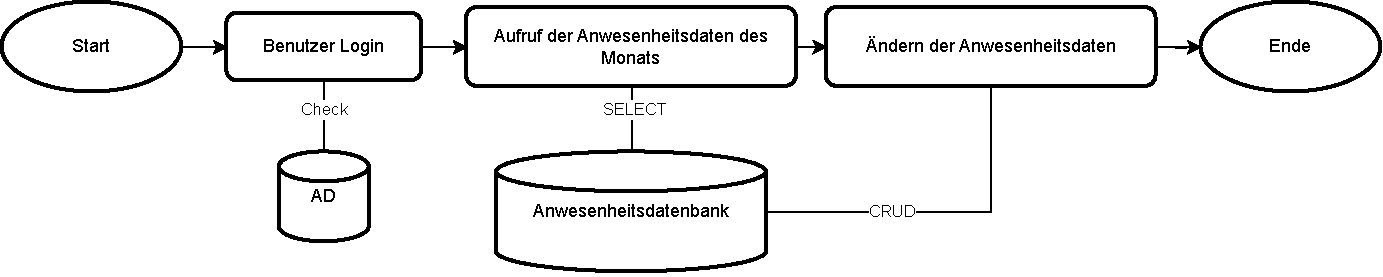
\includegraphics[width=0.9\textwidth,angle=0]{abb/Flow-Diagramm.drawio.pdf}
    \caption[Beschreibung]{Ablaufdiagramm}
    \label{abb:Flow}
\end{figure}

\subsection{Softwaredesigne}
\label{sec:Softwaredesigne}
%TODO: Die sicherheitsstandarts noch refernezieren
Für die Umsetzung des Logikentwurfs mit dem Blazor Framework soll eines der beiden in Absatz \ref{sec:Framework} \nameref{sec:Framework} aufgezeigten Muster implementiert werden. Es konnten sowohl mit MVC als auch mit MVVM bereits Erfahrungen gesammelt werden und deshalb wurde die Entscheidung für ein Muster hauptsächlich aus individuellen Gründen getroffen. Das MVVM Muster ist übersichtlicher und wurde in anderen Projekten bereits erfolgreich umgesetzt. Dasswegen fiel die Wahl auf den einsatz des MVVM Musters.

Damit ergibt sich die Strukturierung des Softwarekomponenten die für das Projekt benötigt werden. Es werden Model Klassen benötigt die, die Anwesenheitsdaten repräsentieren und in der Datenbank persistent gespeichert werden. Das ViewModel ist ebenfalls eine Klasse die, die gesamte Funktionalität für eine View beinhaltet. Damit wird pro View ein ViewModel erstellt. Die View ist nur für die Darstellung zuständig und ist ein HTML Tamplate in das dynamisch Werte aus dem ViewModel gerendert werden.
%TODO:Quelle:https://learn.microsoft.com/de-de/dotnet/architecture/maui/mvvm

Für eine bessere übersicht und ggf. wiederverwendbarkeit von Code sollen für die Datenbankkommunikation und die AD integration eigene bzw. vorhandene Bibliotheken verwendet werden die dann im ViewModel verwendet werden. Für die AD Abfragen soll eine Klassenbibliothek AD Manager erstellt werden und für die Datenbankkommunikation eine DataAccessLibrary. Diese Datenbankkommunikationsbiblithek soll dann die Grundlage für die Datenbankoperationen wie Laden oder Speichern von Daten in der Geschäftslogik sein. In der Geschäftslogik werden diese Methoden zu Laden oder Speichern mit einem SQL Befehl und Objekten an diese Bibliothek übergeben und diese übernimmt dann die Datenbankkommunikation. Das auslagern dieser Basisfunktionalität hat den Vorteil, dass es in anderen Projekten wieder eingesetzt werden kann.

\subsection{Systementwurf}
\label{sec:Systementwurf}
In der Vorbetrachtung wurde sich für die monolithische Systemarchitektur entschieden, da diese einfach Aufzubauen ist und den geringsten Komplexitätsgrad alles Systemarchitekturen aufweist. Dadurch vereinfacht sich die Entwicklung und die Tests, da alle Komponenten innerhalb einer einzigen Anwendung zusammengefasst werden. Eine Skizze des entsteheden Gesamtsystems siehe Anhang \ref{abb:Systemarchitektur}.

Der Webserver auf dem die WebApp läuft bildet das Zentrum des Systems. Um diesen bereitzustellen gäbe es verschiedene Optionen. Docker könnte in Betracht gezogen werden, da die Anwendung dort einer isolierte und portable Umgebung, unabhängig von der zugrunde liegenden Serverkonfiguration ausgeführt werden könnte. Das bereitstellen der WebApp als Container ist in der Infrastruktur des SMK jedoch nur wenig sinnvoll. Zum einen besteht kein Server der Docker Container bereitstellen kann zu andern kann das bereitstellen von Diensten die Anbindung an das AD benötigen für Probleme sorgen. Dementsprechend muss ein Webserver als Host erstellt werden. Dort eignet sich im Kontext des SMK ein IIS Server, dieser auf einem bereits vorhandenen Windows Server installiert werden kann.

Der IIS Server von Microsoft ist der einzige der für das Hosten von Blazor Server WebApps mit ASP.NET Core in frage kommt, da das Framework ASP.NET SignalR zur Kommunikation zwischen Client und Server nutzt. SignalR ist eine von Microsoft entwickelte Bibliothek, die Echtzeit-Webfunktionalitäten in Webanwendungen ermöglicht. Mit SignalR kann eine bidirektionale Kommunikation zwischen Webserver und Webclient herstellen die WebSocket-Verbindungen nutzt um effiziente Verbindung herzustellen. Damit ermöglicht SignalR eine zuverlässige Echtzeit-Kommunikation zwischen Server und Client. (vgl. \cite{SignalR}, \cite{SignalRPlatf})

Die Datenbank als zentrales Speichermedium, sollte im Datenbankcluster des SMK betrieben werden. Für Datenbankserver gibt es im SMK ein eigenes Netz was durch Firewalls speziell abgesichert wird. Da nur der Server eine Verbindung zur Datenbank benötigt um die Daten abzurufen kann nur er durch die Firewall auf den Server zugreifen. Clients haben keine Möglichkeit die Datenbank zu erreichen. Damit wird die Datensicherheit deutlich erhöht. Als Datenbankmanagementsystem (DBMS) werden im SMK nur Microsoft SQL Server betrieben. Um der Vorgabe, möglichst vorhandene Infrastruktur zu nutzen folge zu leisten, wird die Datenbank auf einem SQL Server laufen.

Für die Authentifizierung und Autorisierung der Benutzer wird das bereits bestehende Active Directory des Freistaates Sachsen verwendet. Der Webserver ist in die vorhandenen Domäne des SMK integriert, wodurch eine Authentifizierung am IIS mittels Windows Login durchgeführt werden kann.

\subsection{Datenentwurf}
\label{sec:Datenentwurf}
Um die Daten aus dem Anwesenheitsplaner in eine Datenbank zu speichern muss dafür eine neue, mit passendem Schema, Angelegt werden. UML-Diagramme wie das ERM können dabei verwendet werden, um die Tabellenstruktur, die Beziehungen zwischen den Tabellen und die Attribute zu modellieren. Dies ermöglicht eine klare Darstellung der Datenbankstruktur und hilft dabei, die Datenintegrität und -konsistenz schon in der Planung sicherzustellen. Durch diese Art an Dokumentation ist es auch möglich bei der Entwicklung des Programms passende Klassen für die Verarbeitung der Daten aus der Datenbank herzuleiten.

Die zu speicherten Daten ergeben sich aus der in der Analysephase erhoben Tabelle im Abbildung \ref{abb:Ausgangstabelle}. Um die Daten möglichst simpel aus der Datenbank auslesen und zurückschreiben zu können, sollte versucht werden die Datenstruktur so anzulegen das die Daten in einem in der Programmlogik gut verarbeitbares Schema gespeichert werden. Um möglichst einfache Abfragen zu ermöglichen wurde keine Normalisierung der Tabellenstruktur durchgeführt um Zeit zu sparen. Um später Fehler zu vermeiden könnte das Schema für eine weiterentwicklung angepasst werden. Im aktuellen Fall wurde sich gegen eine Normalisierung entschieden, da die Prüfung der eingaben auf der Frontendseite geschehen soll.

Für das Anlegen der Datenstrukturen im Programmcode und in der Datenbank wurde ein Entity-Relationship-Modell (ERM), siehe \ref{abb:ERM} erstellt. Hier soll es zwei Tabellen geben, die Tabelle Person wird zum Teil aus dem AD befüllt und hält zum Teil Informationen die für Funktionen des Anwesenheitsplaners benötigt werden. Die Tabelle Anwesenheit beinhaltet alle Anwesenheitseinträge der Nutzer. Dem Nutzer wird eine ein Anwesenheitseintrag über die Verbindung mit seinem Sicherheitsbezeichner (SID) im AD zugeordnet. Die SID wird benötigt da sich der Name des Nutzers ändern kann und damit nicht als Primärschlüssel eignet. Die SID wird vom AD beim erstellen des Kontos angelegt und ändert sich nie. (vgl. \cite{sid})

\begin{figure}[htbp]
    \centering
    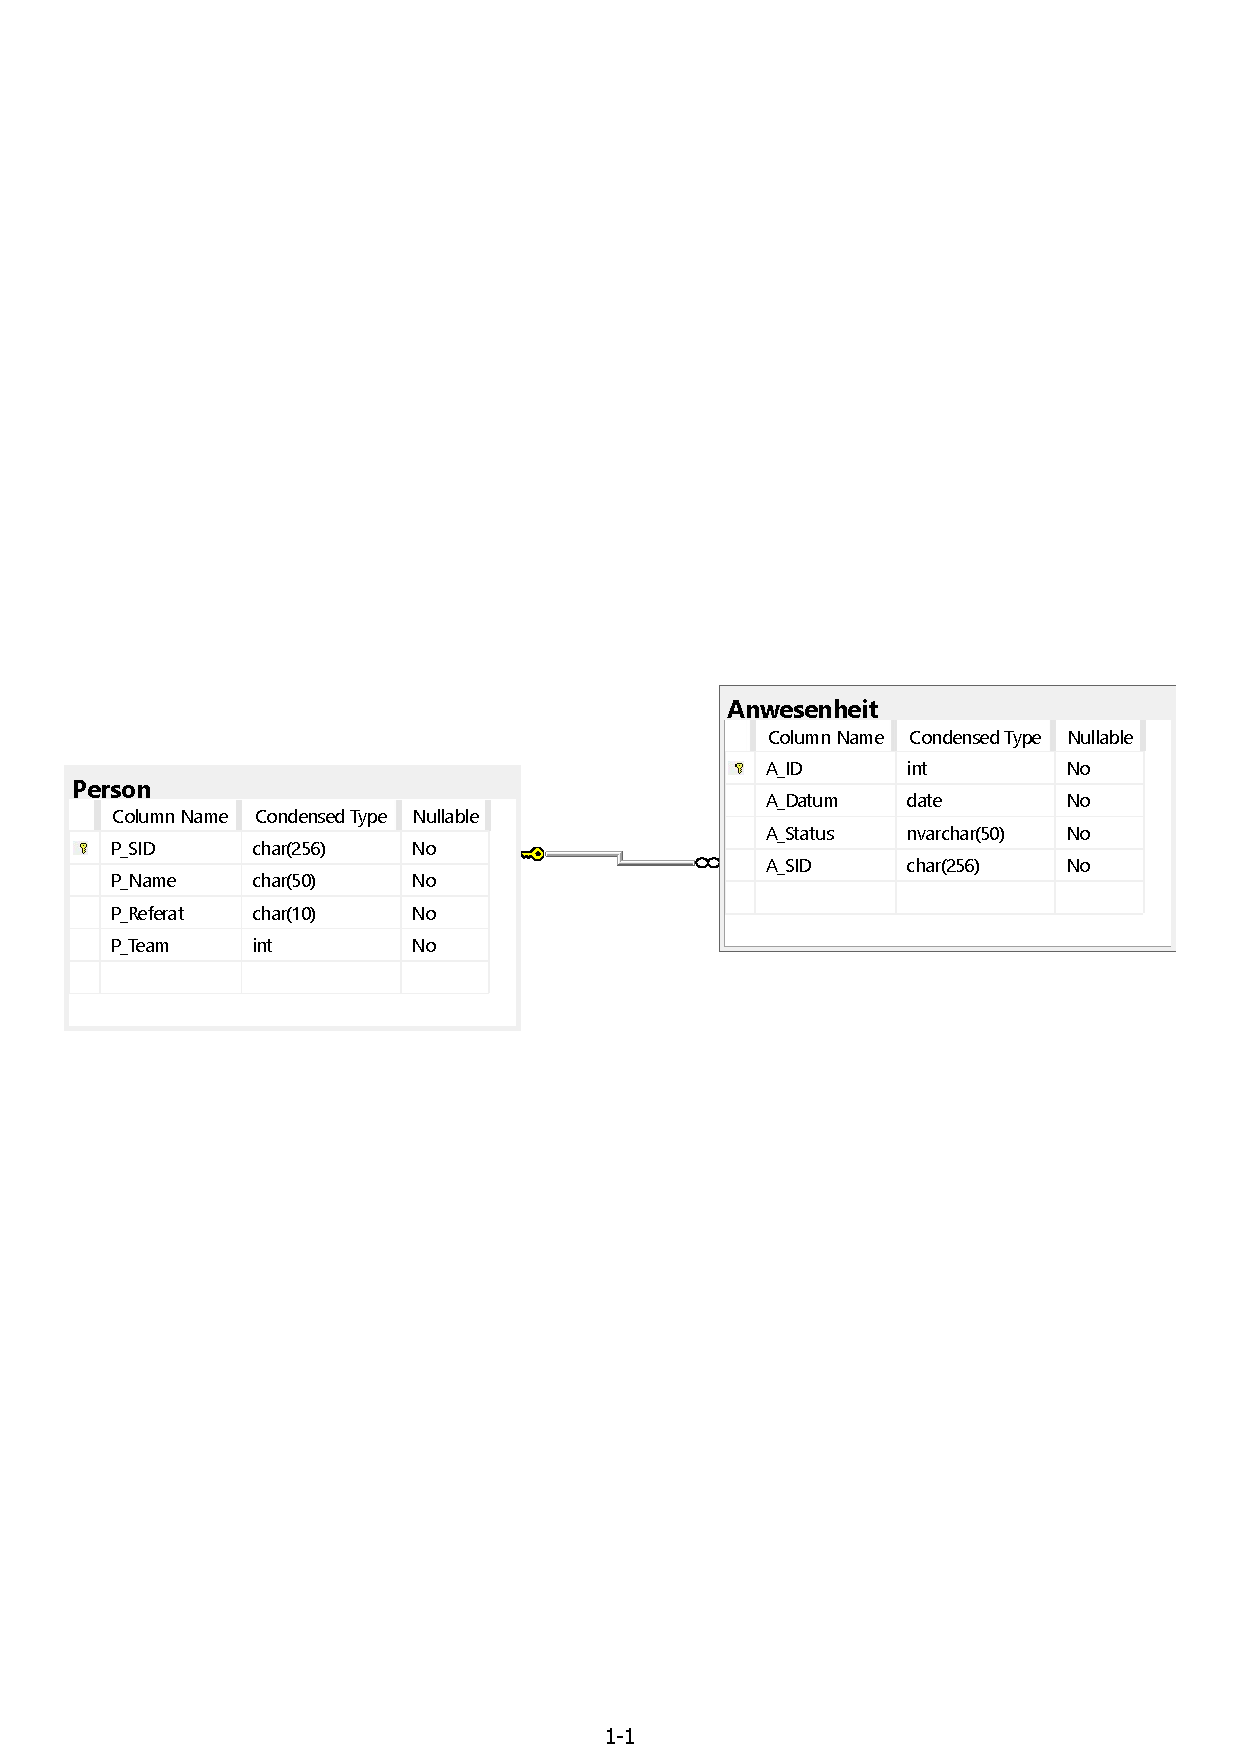
\includegraphics[width=0.9\textwidth,angle=0]{abb/ERM.pdf}
    \caption[Beschreibung]{ERM}
    \label{abb:ERM}
\end{figure}
%TODO:ERM erklären mit Quelle?

